\documentclass[a4paper,12pt]{article}
\usepackage[utf8]{inputenc}
\usepackage[T1]{fontenc}
\usepackage[spanish]{babel}
\usepackage{graphicx}
\usepackage{url}
\usepackage{geometry}
\usepackage{float}
\usepackage{amsmath}
\usepackage[version=4]{mhchem} 
\usepackage{hyperref}
\geometry{top=2.5cm, bottom=2.5cm, left=2.5cm, right=2.5cm}

\begin{document}

\begin{titlepage}
    \centering
    \vspace*{1cm}
    {\huge \bfseries Trabajo Final de Química Computacional\par}
    \vspace*{2cm}
    {\Large Semestre 2024-2\par}
    \vspace{2cm}
    {\large Autor: Emanuel Cabrera Novoa\par}
    \vfill
    {\large Universidad de Medellín\par}
    \vspace{0.8cm}
    {\large Octubre 2023\par}
\end{titlepage}

\section*{Introducción}
En este documento se resolverán los diferentes enunciados del final de Química Computacional I, abordando cada uno de los problemas planteados de manera detallada. Este trabajo tiene como objetivo consolidar los conocimientos adquiridos durante el semestre y aplicar las técnicas de resolución de problemas en química computacional.

\section{Punto 1}
\subsection*{Enunciado}
El hierro puede formar complejos, usando grupos ciano, \ce{(CN)^-1\linebreak}, como ligandos, formado así el complejo
\ce{[Fe(CN)6]^4-}, llamado también Ferricianuro. El espectro de absorción del Ferricianuro se encuentra en el siguiente enlace:  
\url{https://www.metrohm.com/content/metrohm/en/applications/application-notes/dropsens-applikationen-andropsens/an-sec-003.download.pdf}.  
De acuerdo con el espectro de absorción, indique qué color se observa para el complejo \ce{[Fe(CN)6]^3-}. Explique. Luego, consulte qué es el azul de Prusia, su historia, cómo se obtiene y cuál es la fórmula. Consulte el espectro de absorción del azul de Prusia y explique por qué se observa su color característico.

\subsection*{Solución}
\section*{Color del Complejo \ce{[Fe(CN)6]^{3-}}}
El complejo \ce{[Fe(CN)6]^{3-}} presenta color debido a la absorción de luz en el espectro visible. Según su espectro de absorción, este compuesto muestra un pico alrededor de los 420 nm, lo que indica una fuerte absorción en la región azul-violeta del espectro visible.

La causa del color observado es la excitación de electrones desde su estado fundamental a niveles de energía más altos. Aplicando la teoría del color complementario:
\begin{itemize}
    \item El complejo absorbe luz azul-violeta.
    \item El color complementario al azul-violeta es amarillo-naranja.
    \item Por lo tanto, el complejo aparece de color amarillo-naranja.
\end{itemize}
\section*{Azul de Prusia}

\subsection*{Historia}
El Azul de Prusia marcó un hito en la historia de los pigmentos sintéticos. Fue descubierto accidentalmente en Berlín en 1704 por Heinrich Diesbach mientras intentaba producir un pigmento rojo utilizando cochinilla, sulfato ferroso y potasa. En su lugar, obtuvo un intenso color azul.

El nombre del compuesto proviene de su uso en los uniformes del ejército prusiano en el siglo XVIII, aunque también es conocido como Azul de Berlín, Azul de París o Azul de Turnbull. Curiosamente, fue uno de los colores originales de los crayones Crayola en 1903, hasta ser reemplazado por Azul Medianoche en 1958. Es un pigmento azul oscuro con un matiz verdoso, considerado el primer pigmento sintético moderno.

\subsection*{Estructura química}
Químicamente, el Azul de Prusia tiene una fórmula empírica \ch{Fe7(CN)18}, pero se representa más precisamente como \ch{Fe4[Fe(CN)6]3}. Esto refleja la presencia de dos estados de oxidación distintos del hierro. Cada unidad de fórmula puede incorporar hasta 16 moléculas de agua y contener impurezas inorgánicas que afectan su tono.

Estructuralmente, contiene aniones \ch{[Fe(CN)6]^{4-}} con geometría octaédrica, formando una red cristalina cúbica donde los iones están conectados por puentes de cianuro. Su síntesis implica una reacción redox entre sales férricas (\ch{Fe^{3+}}) y ferrociánicas (\ch{Fe^{2+}}).

El Azul de Prusia debe su color azul profundo a patrones específicos de absorción en el espectro visible:
\begin{itemize}
    \item Fuerte absorción en el rango de 600-700 nm (región naranja-roja).
    \item Esta absorción resulta de una transferencia de carga entre \ch{Fe^{2+}} y \ch{Fe^{3+}} a través de los puentes de cianuro.
    \item Al absorber luz naranja-roja, se observa su color complementario: azul.
\end{itemize}

La intensidad del color azul se ve potenciada por:
\begin{itemize}
    \item Alta absortividad molar del complejo.
    \item Eficiente transferencia de carga entre los centros de hierro.
    \item La estructura cristalina cúbica regular.
\end{itemize}

La absorción en la región naranja-roja elimina estas longitudes de onda de la luz blanca, dejando principalmente las longitudes de onda azules (400-490 nm) para ser reflejadas o transmitidas, lo que genera el característico color azul intenso.

\section{Punto 2}
\subsection*{Enunciado}
Visualizar y mencional elementos de simetría del ciclobutano, usando la herramienta \textit{symotter}. Establecer el grupo puntual de simetría con diagrama de flujo usado en clase o similares. Consultar tabla de caracteres. Asignar cuántos modos normales de vibración hay en cada caso. Explique.
\subsection*{Solución}
\subsection{Elementos de Simetría del Ciclobutano}

\subsubsection{Identidad}
La identidad es la operación de simetría más simple y fundamental en química. Representa el estado en el que una molécula permanece completamente sin cambios. El ciclobutano tiene a la identidad como parte de su grudo de simetría. 
\subsubsection{Reflexión}
La reflexión implica "voltear" cada punto de un objeto o molécula sobre un plano especular, de modo que la distancia de cada punto al plano sea la misma, pero en direcciones opuestas.
\subsubsection{Plano horizontal}
El ciclobutano tiene un único plano horizontal de reflexión.
\begin{figure}[!ht]
	\centering
	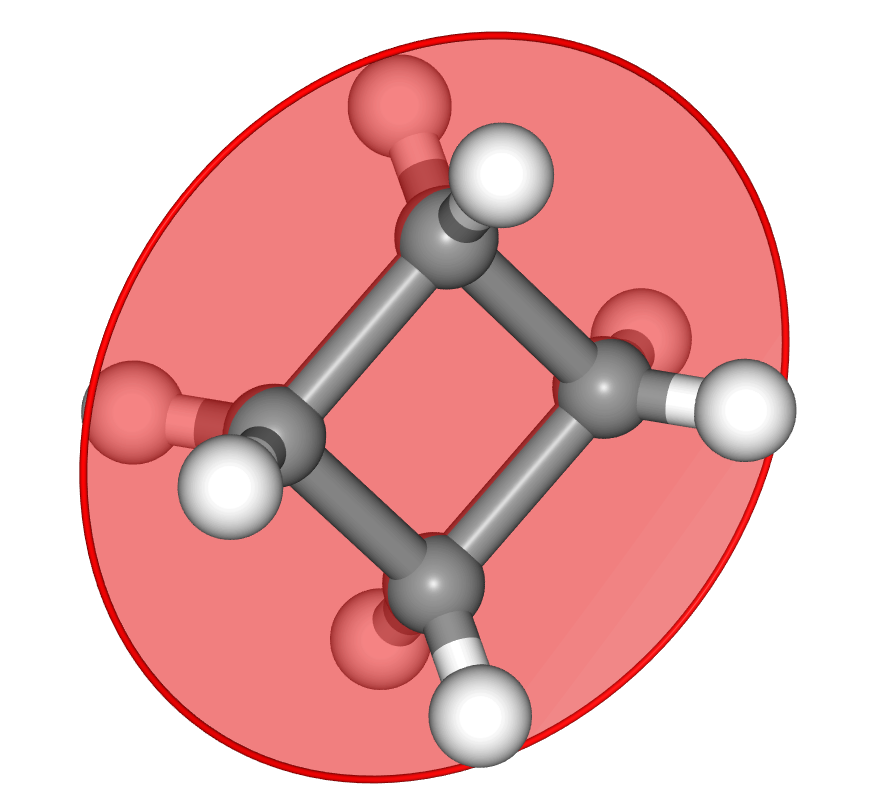
\includegraphics[width=0.45\textwidth]{./media/plano_horizontal_1.png}
	\caption{$\sigma_h$ reflection}
\end{figure}
\subsubsection{Planos Vertical}
El plano de reflexión contiene el eje principal de simetría. El ciclobutano tine dos planos verticales de reflexión. 
\begin{figure}[H] 
\centering
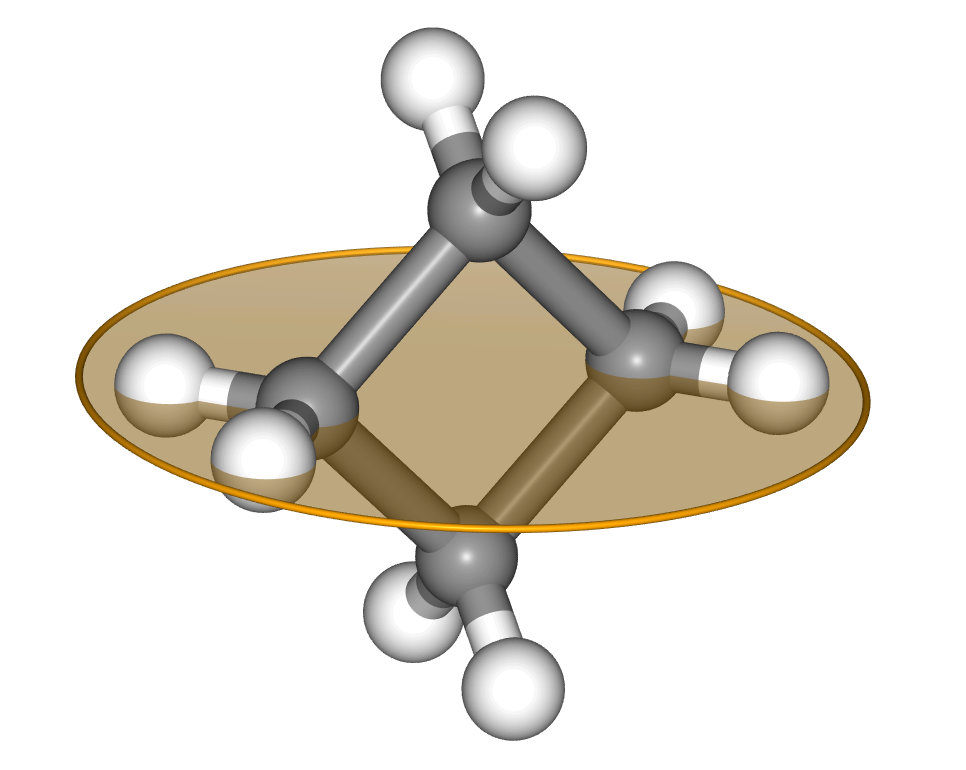
\includegraphics[width=0.45\textwidth]{./media/reflexion_vertical_1.png}
\hfill
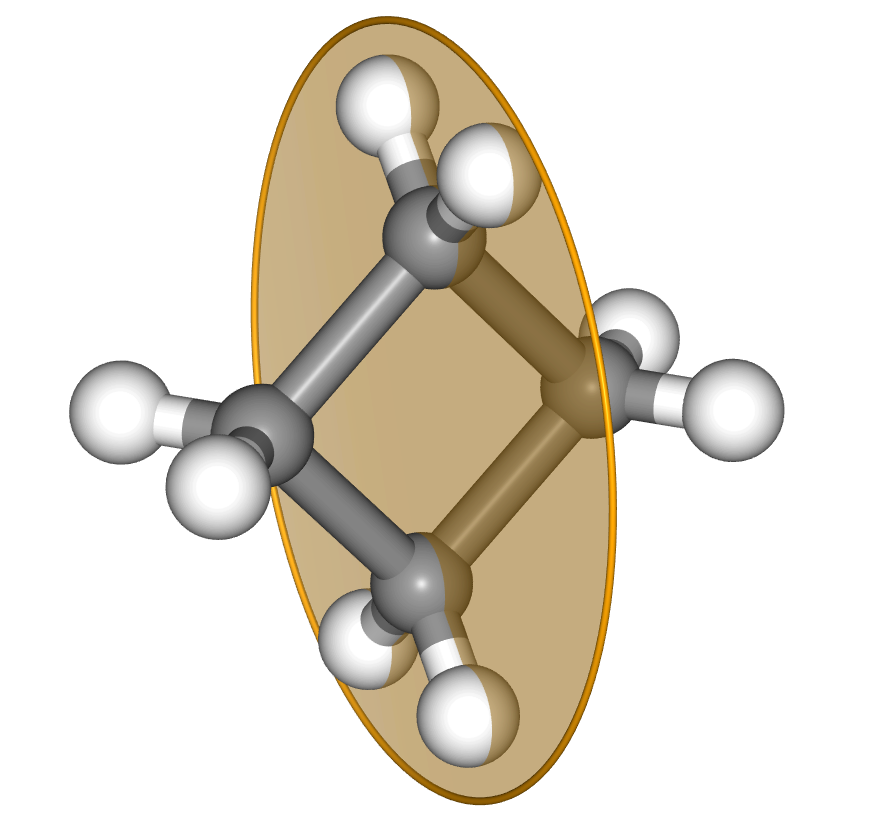
\includegraphics[width=0.45\textwidth]{./media/reflexion_vertical_2.png}
\caption{$\sigma_v$ reflection}
\end{figure}
\subsubsection{Plano Diagonal}
Es un subtipo de $\sigma_v$ que incluye planos que dividen los ángulos fomardos pr los elementos de simetría.
\begin{figure}[H]
	\center
	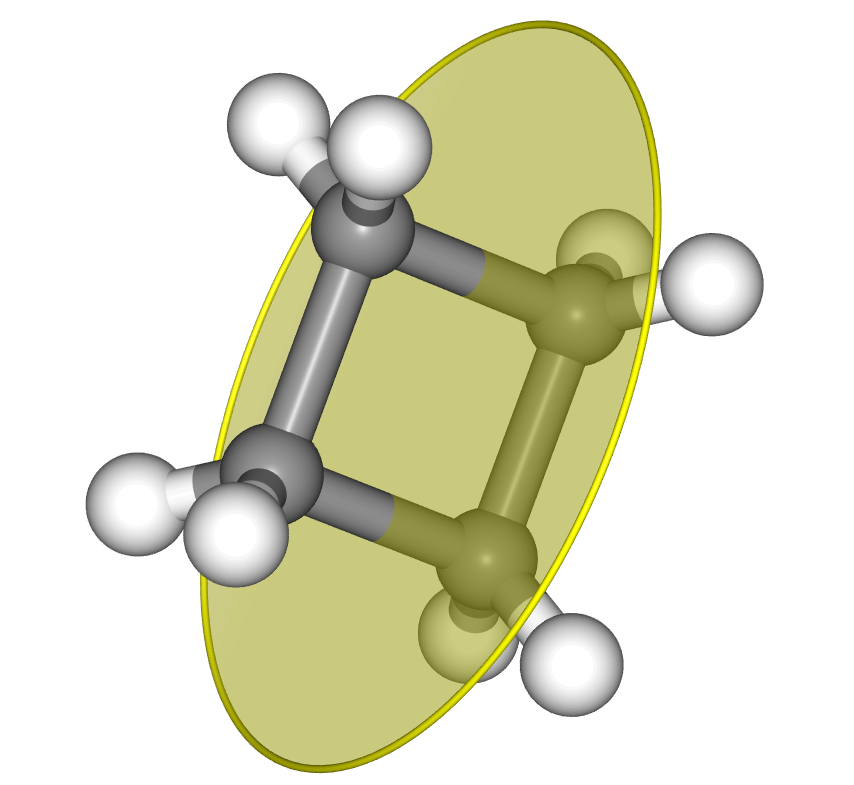
\includegraphics[width=0.45\textwidth]{./media/relfection_diagonal_1.png}
	\hfill
	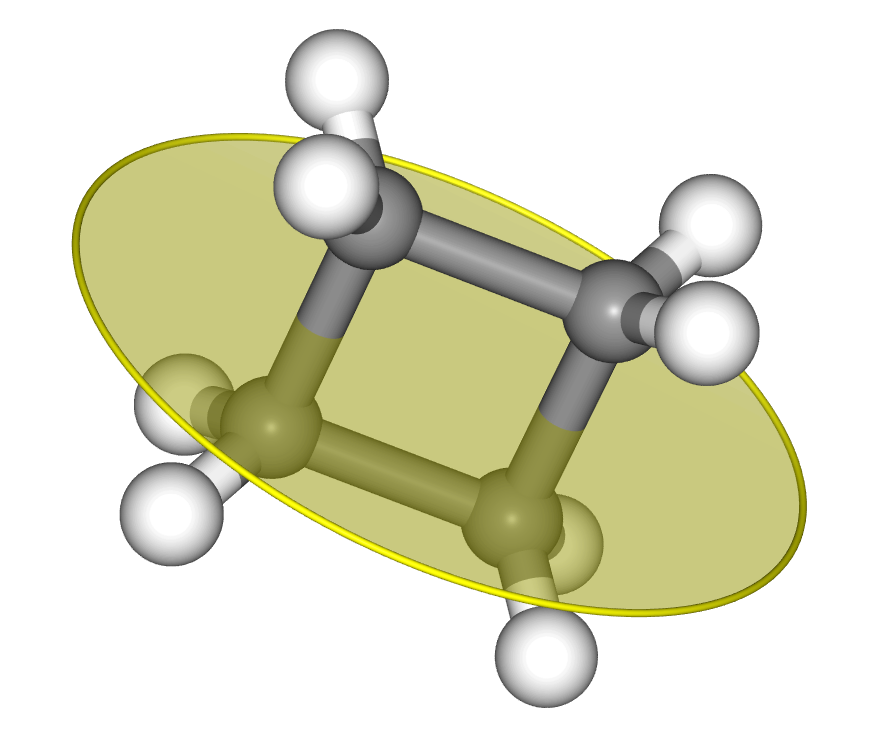
\includegraphics[width=0.45\textwidth]{./media/reflection_diagonal_2.png}
	\caption{$\sigma_d$ reflection}
\end{figure}

\subsubsection{Inversión}
La inversión implica refljar todos los puntos de una molécula con respecto a un \textbf{centro de inversión}. El ciclobutano tine un único centro de inversión.
\begin{figure}[!ht]
	\center
	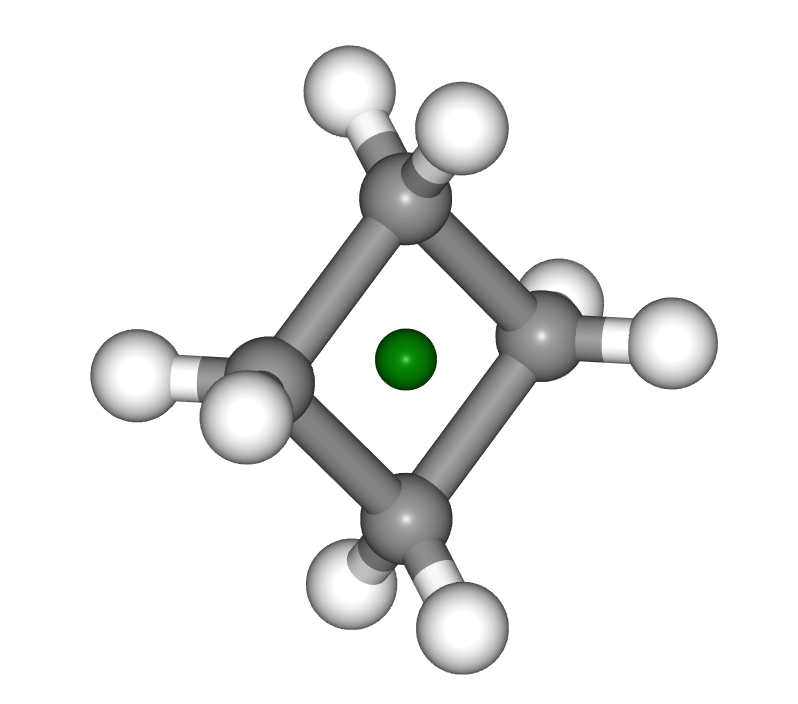
\includegraphics[width=0.45\textwidth]{./media/inversion.png}
	\caption{inversión}
\end{figure}
\subsubsection{Rotación Propia}
La rotación propia describe la capacidad de una molécla para superponerse consigo misma despues de rotar de un \textbf{eje de simetría} (eje de rotación propio). Para el ciclobutano temos:
\begin{itemize}
	\item Un (1) eje de rotación $C_4$
	\item Cinco (5) ejes de rotación $C_2$
\end{itemize}
\begin{figure}[!ht]
	\center
	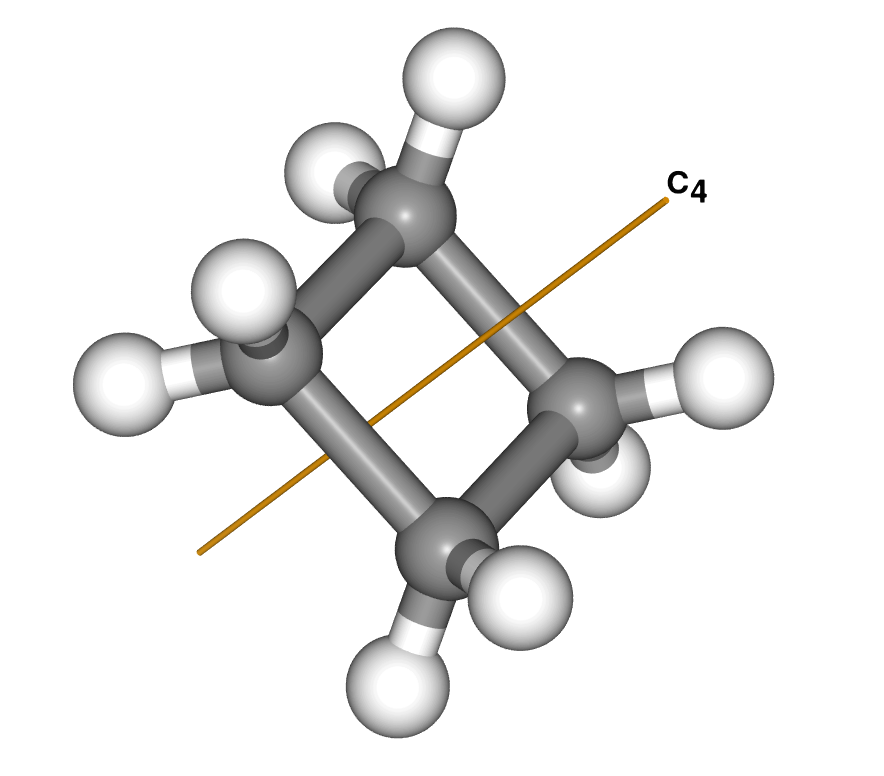
\includegraphics[width=0.45\textwidth]{./media/rotacion_propia_1.png}
	\caption{Rotación Propia ($C_4$)}
\end{figure}
\begin{figure}[!ht]
	\center
	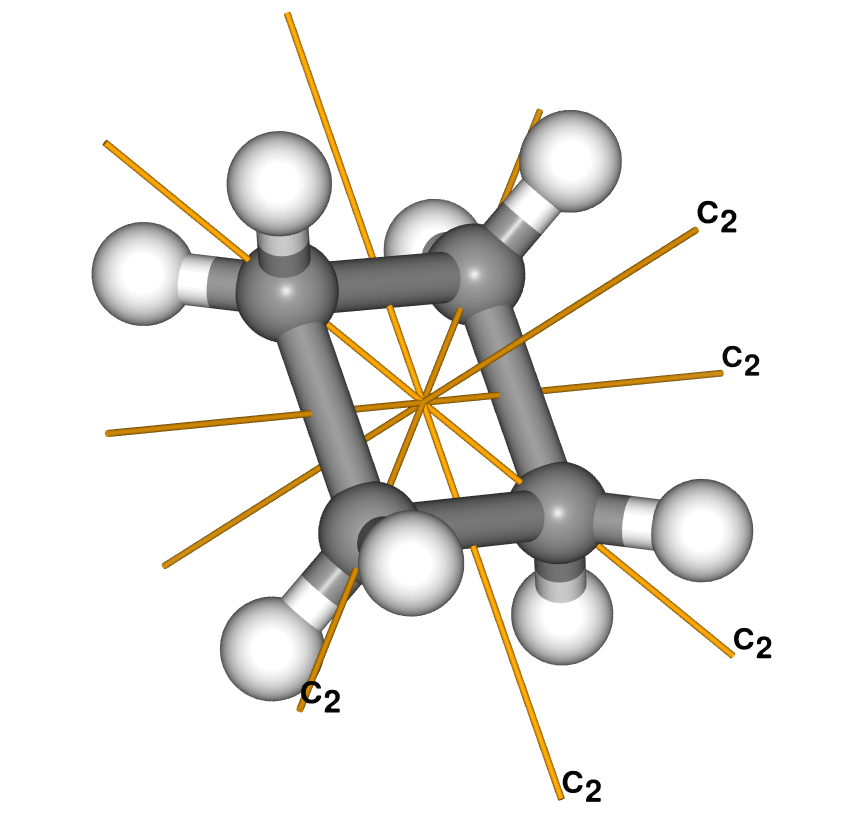
\includegraphics[width=0.45\textwidth]{./media/rotacion_propia_2.png}
	\caption{Rotación Propia ($C_2$)}
\end{figure}
\subsubsection{Rotación Impropia}
La rotacióm impropia es una operación de simetría que combina dos transformaciones: una \textbf{rotación propia} seguida de una \textbf{reflexión} en un plano perpendicular al eje de rotación. El ciclobutano tiene una sola rotoación impropia.
\begin{figure}
	\center
	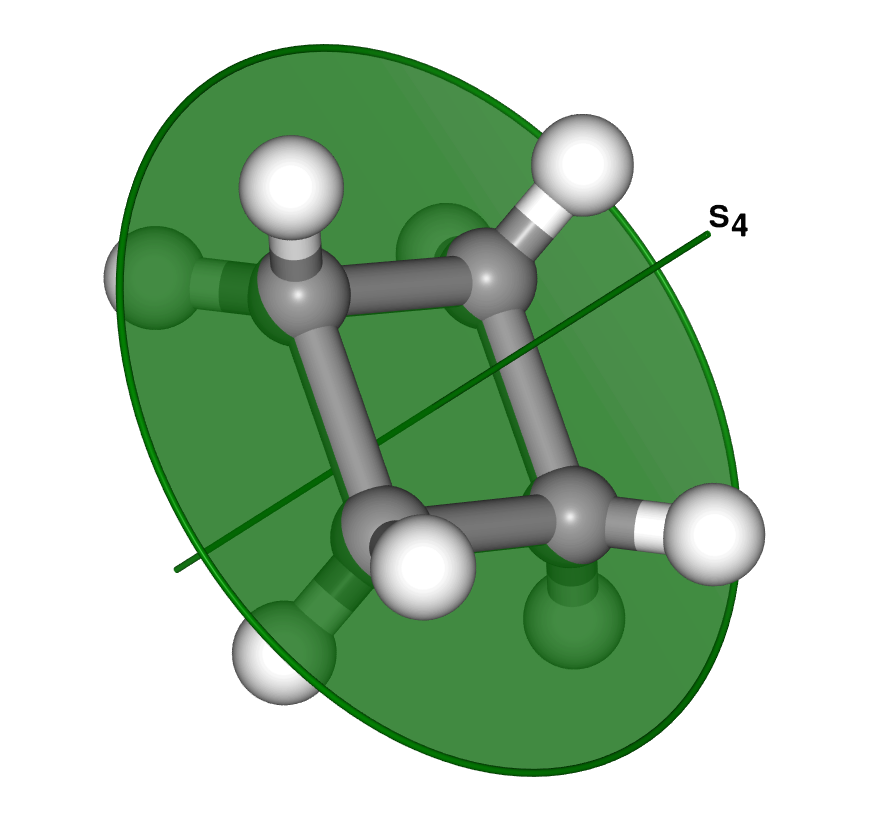
\includegraphics[width=0.45\textwidth]{./media/rotacion_impropia.png}
	\caption{Rotación Impropia ($S_4$)}
\end{figure}
\subsection{Grupo Puntual de Simetría del Ciclobutano}
Ya optenidos los elementos de simetría del ciclobutano, el siguiente paso para conocer le grupo puntual de simetría es utilizar el diagrama de flujo de grupos puntuales e ir respondiendo las preguntas una a una.
\begin{figure}[!ht]
	\center
	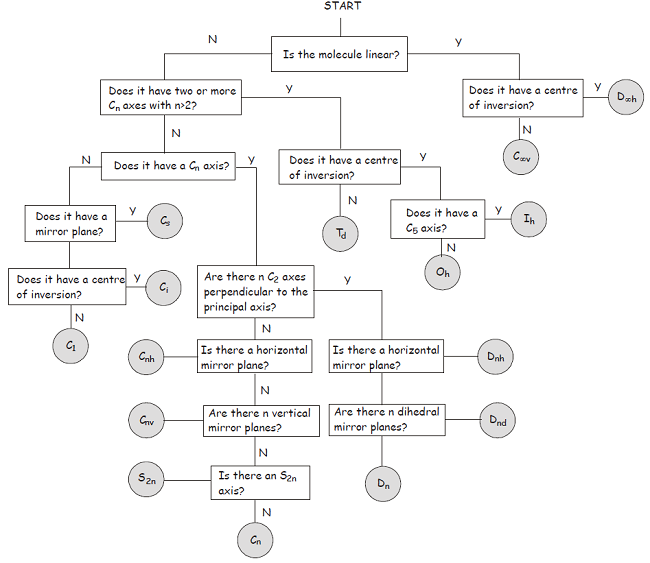
\includegraphics[width=0.45\textwidth]{./media/grups_puntuales_de_simetria.png}
	\caption{Diagrama de flujo de los grupos puntuales de simetría}
\end{figure}
\begin{itemize}
\item \textbf{¿La molecula es lineal?:} No
\item  \textbf{¿Tiene dos o más ejes $C_2$ con $n>2$?:} No
\item \textbf{¿Tiene eje $C_n$?}: Si
\item \textbf{¿Hay $n$ ejes $C_n$ perpendiculares al eje principal?:} Si
\item \textbf{¿Existe un plano de espejo horizontal?:} Si
\item \textbf{Resultado:} $D_{4h}$
\end{itemize}
\subsection{Modos Normarles de vibración del Ciclobutano}
\subsubsection{Grados de libertad totales}
El ciclobutano tiene cuatro (4) átomos de carbono y ocho (8) de hidrógeno, lo que da un total de doce (12) átomos. Cada átomo tiene 3 grados de libertad (traslación en $x$, $y$, $z$), así que el total es:
$$
3 \times 12 = 36 \text{ grados de libertad}
$$
\section{Punto 3}
\subsection*{Enunciado}
Realizar optimización de la molécula usando \textit{chemcompute.org}, usando las siguientes opciones: IR, Geometry, Optimization y dejando el resto de opciones elegidas por defecto. Elija un modo vibracional de su elección, cuyo numero de onda es --- $cm^{-1}$ y describa el tipo de vibración observada. Obtenga el potencial electro estático respectivo y explíquelo.
\subsection*{Solución}
\subsubsection{Análisis Vibracional}
En el presente análisis vibracional del ciclobutano, se seleccionó una frecuencia específica de 23.65 $cm^{-1}$, la cual corresponde a un modo vibracional de tipo \textbf{torsión}. Este tipo de vibración se carateriza por el movimiento relativo de llos átomos entorno a un eje, sin un cambio significativo en las distancias de enlaces.
\subsubsection{Análisis del Densidad Electroestática}
\subsubsection*{Distribución de Densidad Electrónica}
La escala de colores varía de -0.10 (rojo) a 0.04 (azul):
\begin{itemize}
	\item \textbf{Regiones rojas y anaranjadas:} Indican áreas de mayor densidad de carga negativa asociadas a los enlaces C-H más electronegativos.
	\item \textbf{Regiones verdes y azules:} Representan áreas de menor densidad de carga o incluso positivas, conmúnmente asociadas a los centros de los enlaces C-C donde la densidad electrónica está más distribuida.
\end{itemize}

\begin{figure}
	\center
	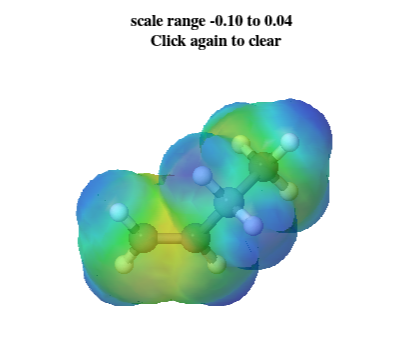
\includegraphics[width=0.45\textwidth]{./media/potencial_electroestatico.png}
	\caption{Potencial electroestático para la frecuencia de vibración 23.65 $cm^{-1}$}
\end{figure}
\section{Punto 4}
\subsection*{Enunciado}
Use Materials Project y la API respectiva, además Colab o Jupyter, para importar la perovskita Ca-Ti. Incluya un resumen de lo que usted ya realizó durante el semestre en una tabla, donde se indique los artículos más relevantes del tema que incluya i) el títul de los artículos, ii) la revista, iii) el factor de impacto y iv) el cuartil (Q1, etc.) 
\subsection*{Solución}
El siguiente es un enlace a un Colab con la respuesta del punto 4: \url{https://colab.research.google.com/drive/10yBal99DN2I6t3--xiFXwM0rT9GmUJhm?usp=sharing} 
\section{Punto 5}
\subsection*{Enunciado}
Para el material asignado, indieque los siguente i) Red de Bravais, ii) mp-ID, iii) notación de Hermann-Mauguin. Explique la notación de Hermann -Mauguin respectiva.
\subsection*{Solución}
\begin{table}[h!]
\centering
\begin{tabular}{lllll}
\toprule
\textbf{Red de Bravais} & \textbf{ID de Materials Project} & \textbf{Fórmula} & \textbf{Grupo Espacial} & \textbf{Notación Hermann-Mauguin} \\
\midrule
Ortorrómbica           & mp-4019                         & \ch{CaTiO3}      & Pbnm                    & $P2_1/m2_1/m2_1/m$ \\
\bottomrule
\end{tabular}
\caption{Propiedades del CaTiO$_3$.}
\label{tab:catioproperties}
\end{table}

\subsubsection{Explicación de la Notación de Hermann-Mauguin para \textit{Pbnm}}
 
La notación de Hermann-Mauguin se utiliza para describir la simetría de los grupos espaciales cristalográficos. En este caso, consideramos el grupo espacial \textbf{Pbnm}, que se puede detallar como $P2_1/m2_1/m2_1/m$.

\subsection*{Desglose de la notación completa $P2_1/m2_1/m2_1/m$}

\begin{itemize}
    \item \textbf{P}:
    Indica que la celda es \textit{primitiva}, lo que significa que los puntos reticulares están ubicados únicamente en las esquinas de la celda unitaria.

    \item \textbf{$2_1/m$}:
    \begin{itemize}
        \item \textbf{$2_1$}: Representa un eje helicoidal de simetría de orden 2. Esto combina una rotación de $180^\circ$ con una traslación fraccional a lo largo del eje helicoidal.
        \item \textbf{/m}: Indica la presencia de un plano de reflexión perpendicular al eje helicoidal.
    \end{itemize}

    \item \textbf{Repetición de $2_1/m$}:
    \begin{itemize}
        \item El sistema cristalino ortorrómbico tiene tres direcciones principales ($a$, $b$, $c$), y cada una de estas direcciones está asociada con un conjunto de operaciones de simetría. En este caso, cada eje tiene un eje helicoidal $2_1$ y un plano de reflexión $m$.
    \end{itemize}
\end{itemize}
\section{Punto 6}
\subsection*{Enunciado}
Usando \textit{Pymatgen}, modifique la estructura cristalina así: i) cambie un átomo por otro (incluya átomo de Ti), ii) mueva un átomo 0.9 A en una direcció de su preferencia (x, y, z), iii) elimine un átomo de su preferencia. Para cada caso (i, ii, iii), indique (\textit{print}) el grupo especial resultante. Explique las observaciones realizar.
\subsection*{Solución}
El siguiente redirige a un notebook donde se le da solución al punto 6: \url{https://colab.research.google.com/drive/1m6wo_DTORMPzqj7yUSKnQn9Qw-0sLmvc}
\section{Punto 7}
\subsection*{Enunciado}
Usando \textit{Pymatgen}, identifique materiales compestos por los elementos Ni, Cr y O, que tenga un band gap entre 0.1 y 2.8 eV. Explique sus líneas de código usadas y los resultados obtenidos.
\subsection*{Solución}
El siguiente enlace lleva a un notebook en Colab donde se le da solución al punto 7: \url{https://colab.research.google.com/drive/1B3C2IcFyrpm7PTzQJkTYYQXjpz4YOu0g?usp=sharing}
\section{Punto 8}
\subsection*{Enunciado}
Usando \textit{Matminer}, realice la misma búsqueda del numero anterior (7). Discuta las ventajas y desventajas \textit{Pymatgen} vs \textit{Matminer}.
\subsection*{Solución}
El siguiente enlace lleva a un notebook en Colab donde se le da solución al punto 8: \url{https://colab.research.google.com/drive/1LhMufZ6e8725Tnrnm27HsOyian_Xdw8N?usp=sharing}
\section{Punto 9}
\subsection*{Enunciado}
Contruya una nanopartícula de Au, usando las siguientes energías libres libres de superficie (eV/$A^2$): 2.1, 2.0, 1.9, asignándolas para las tres superficies de mayor intensidad que usted encuentra en Materials Project. Use un tamaño de 100 átomos. Luego de realizar la construcción de Wulff, asigne un tamañ de 300 y 500 átomos. Mida el tamaño de cada nano partícula (100, 300, 500 átomos) y discuta al respecto a la \textit{facilidad} vs \textit{realidad} del modelo a usar, pensando en na modelación computacional de esas nanopartículas.
\subsection*{Solución}
El siguiente enlace lleva a un notebook en Colab donde se le da solución al punto 9: \url{https://colab.research.google.com/drive/1q8EEW-HvayJtRUlFDYdP1EEOpMC28Vyn?usp=sharing}
\section{Punto 10}
\subsection*{Enunciado}
Use su material de la exposición \#1, cuyo mp-ID es: ---. User PyXtal para identificar los picos más intensos del patrón de difracción y así optener una superficie representativa. Dibuje la superficie, usando varios layers (usted elige, entre 2 y 8) y un vacío de 10 A. la superficie creada por defecto es la (1x1). Identifique la carga de los átomos (positiva y negativa), usando como guía la carga asignada en la ccelda unitaria del sistema respectivo en Materials Project.
\subsection*{Solución}
El siguiente enlace leva a un notebook en Colab donde se le da solución al punto 10: \url{https://colab.research.google.com/drive/1jf2bHDpmeA-bSc-J21qzz68SOPvp1_aG?usp=sharing}
\section{Punto 11}
\subsection*{Enunciado}
Use su sistema analizando en el numeral 2), particularmente el potencial lectrostático. Adicione la molécula sobre la superficie creada en 10), ubicándola en sitios pertinentes de la fuperficie, de acuerdo con criterios de cargas. Una vez incluida la molécula (adsorbato) sobre la superficie (1x1), replique el sistema en x, y y mida la distancia entre adsorbatos (moléculas adsorbidas) de celdas vecinas. si la distancia es menor a 5 A, cree una supercelda más grande, como (2x1), (1x2), (2x2), etc., tal que las distancias entre adsorbatos vecins en x,y sea mayor a 5 A. Discuta respecto al procedimiento realizado, incluyendo i) distancias entre adsorbatos, ii) tamaño de la supercelda obtenida, iii) número total de átooms en el slab. Para este último caso (iii) consulte si la modelación usando DFT sería viable o restrictiva.
\subsection*{Solución}
\end{document}
